%************************************************
\chapter{Analysis and methodology}\label{ch:objectives}
%************************************************

% descripción del proyecto: objetivos, metodología: pasos del diseño y desarrollo, ver figura 3.1 (elección de sensores: computing offloading), contexto (partimos de ABC4T: recordar P2ABCE y que se basa en tarjetas), entorno de desarrollo (meter elección del Omega2, LEDE, teoría de APDUs, código heredado) el sw, los tests p2abce puro, 


%TODO resumir organización del capítulo


In this chapter we describe the project objectives, and the methodology followed during its development. In section ... TODO

\section{Project description}

The purpose of this project is the integration of IBM's privacy preserving solution, Idemix, in the environment of the Internet of Things. The objective is to design a general solution for the existing IoT devices and systems, without compromising any feature of Idemix, and provide a working PoC in a real IoT environment, even though it isn't the most constrained scenario. The project is aimed to be used in privacy preserving environments, providing security for IoT, controlling what data is being disclosed and to whom. In a smart city project, citizens data can be privatized and continue to offer the benefits of the sensors around. Authorized personnel can disclose the information when required, like firefighters that could access a building sensors to know how many people and what conditions they are in, in case of a emergency; and keep such invasive data private to other non-critical services, for example, only giving a proof that there are more than a minimum number of people in the building, to activate or deactivate the air-conditioning system.

\hfil

We will divide the project in various \textbf{objectives}, starting from the principal goal, dividing our work in different categories.

\hfil

\paragraph{Idemix and the IoT}
We part from this main objective, integrating IBM's privacy preserving system in the IoT environment. 

\paragraph{Analysis} Study the state of the art for Idemix and the IoT, analyzing related projects like ABC4Trust's \ac{P2ABCE}, papers with similar approaches, and our task is to consider the best fitting solutions from where to start.

\paragraph{Design and implementation} After studying the existing works, we must give a formal solution to be implemented. This includes the theoretical architecture, the steps to take, the software to implement, the hardware to use, and any simplifications to leave as future work.

Our \textbf{software} objectives include making it easily maintainable, structured and extensible, from the IoT and original project perspectives, that is, the IoT solution must be interoperable with other non-IoT solutions, now and in the future, with minimal effort, given new IoT systems or changes in the cryptographic protocols.

Our \textbf{hardware} objective is to use devices as constrained as possible. But considering our early situation in the project, we will use IoT devices that ease testing and development, having in mind the other devices, and what specific steps we should take for them in the future.

\paragraph{Validity and evaluation} Deploy a \ac{PoC} in a \textbf{real scenario}, without the need of simulators, checking it works as expected, and measuring its performance.



\section{Methodology}

Giving the vast range of IoT devices, a one-for-all solution must take in consideration multiple requirements and limitations. We will break down the original system, Idemix and P2ABCE, analyze every part of it and categorize them. We will consider what components are mandatory to be executed in the target device and which ones the devices would be able to execute.

Devices with equivalent processing power to smart phones are capable to execute the current Java implementations of P2ABCE and Idemix, but the most constrained ones can't handle the entire system, only the key cryptographic operations.

Using the technique known as \textit{Computation Offloading} we will design an IoT architecture where the most constrained targets can keep their private keys and certificates secure in the same device, and act as any other User in the P2ABCE system. Studying the P2ABCE architecture and implementations we will identify those mandatory operations to be executed in the constrained device, and how to communicate efficiently during the delegation.

After the technical design, we will implement the PoC, using software designs patterns known to many professionals, that will improve the maintainability of the project, for improvements and fixes. Taking advantage of this practices, we can document the immediate steps for future developers, how to reimplement certain interfaces when porting the application to a new system, or where the core logic lies for future protocol changes.

Finally, the PoC must be evaluated to assert we achieved our goals, and measure its performance, judging if it could be fitting for real IoT environments.



\section{Analysis of P2ABCE}

% TODO: explicar P2ABCE


In the \ac{P2ABCE} repository \citep{p2abcurl} is available the project's code, divided in two solutions: a complete P2ABCE implementation in Java and a Multos Smartcard implementation as companion for the project.

The Java code is managed by a Maven project, structured using various known design patterns, but not of our interest. The structure we are actually interested in are the REST Services and their use of the Components classes, in which the smartcards are included.

P2ABCE project is based on the concept of smartcards to store the credentials, logical or physical. An interface is defined to communicate with these smartcards, and then different implementations allow to use either \textit{Software Smartcards} or \textit{Hardware Smartcards}. 

The \textit{SoftwareSmartcard} class implements the interface in Java, suitable for tests and self-stored smartcards that any application using P2ABCE may need.

The \textit{HardwareSmartcard} class uses the standard APDU messages [TODO:ref] to interact with smartcards. P2ABCE defines for every method in the mentioned interface, the necessary APDU instructions, and currently relies on \textit{javax.smartcardio} abstract classes (implemented by Oracle in their JRE) to communicate with the smartcard reader. This way, it doesn't matter what manufacturer issues the smartcard, or if it's an Android device, if they support the APDU API, P2ABCE will work with them.

\begin{figure}[bth]
	\begin{center}
		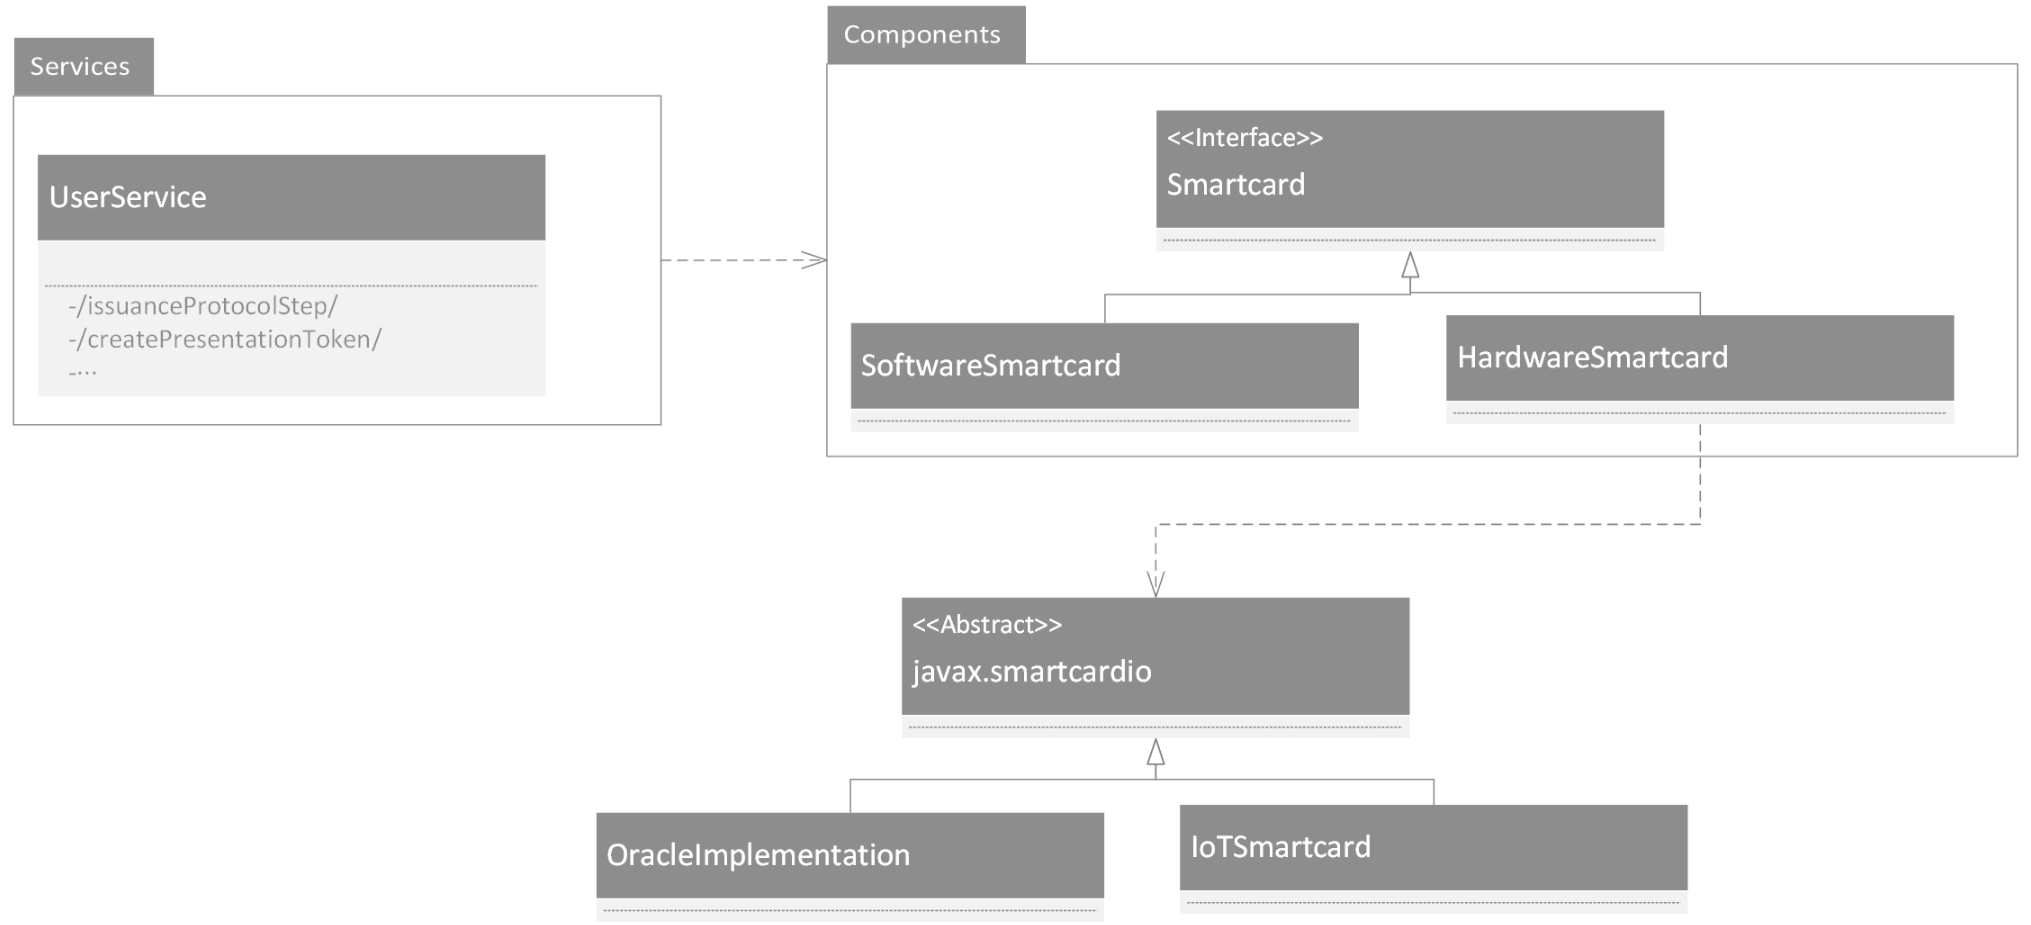
\includegraphics[width=\linewidth]{gfx/p2abceBasicUML}
	\end{center}
	\caption{Basic P2ABCE structure}
	\label{fig:p2abceBasicUML}
\end{figure}


As a PoC the P2ABCE project includes the ABC4Trust Card Lite, an implementation for ML3-36K-R1 Multos Smartcards. The code is written in C, but is very dependent on the Multos framework, aside from numerous bugs and bad coding habits. 



At this stage, we have two options to implement our IoT device compatible with P2ABCE:

\begin{itemize}
	\item Implement in C the \textit{Smartcard} interface used by P2ABCE architecture, and use some communication protocol to remotelly call the methods from the machine running the P2ABC Engine.
	\item Present the IoT device as a hardware smart card, using the APDU protocol (already defined, standard and with minimal overload). Providing a \textit{javax.smartcardio} ``IoT implementation'' to communicate with the IoT device through a transmission protocol, the already existing \textit{HardwareSmartcard} class can work with the new \textit{IoTSmartcard} in the IoT device.
\end{itemize}



\subsection{ABC4Trust Card Lite}

%TODO: as part of P2ABCE project, this MULTOS PoC

%TODO: check content

P2ABCE provides a smart card reference implementation, ABC4Trust Card Lite \citep{ABC4TCardLite}. It supports device-bound U-Prove and Idemix, and virtually any discrete logarithm based pABC system.

Version 1.2 is based on MULTOS ML3 cards, with approximately 64KB of EEPROM (non-volatile memory), 1KB of RAM and an Infineon SLE 78 microcontroller, a 16-bit based CPU aimed for chip cards.

The card stores the user's private key $x$ and any \ac{BLOB} that the P2ABCE may need (like user's credentials). Then P2ABCE delegates the cryptographic operations on the smart card, that operates with $x$.

\begin{figure}[bth]
	\begin{center}
		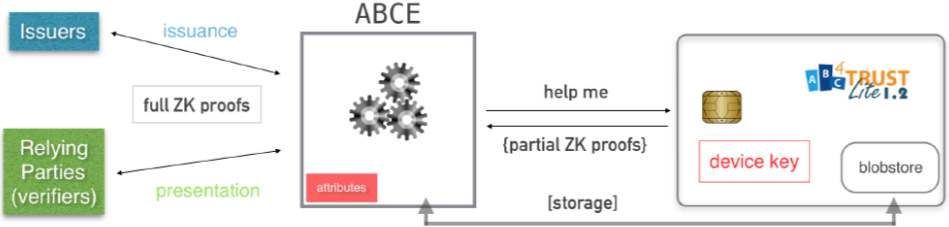
\includegraphics[width=\linewidth]{gfx/ABC4TCardLite}
	\end{center}
	\caption{ABC4Trust Card Lite}
	\label{fig:ABC4TCardLite}
\end{figure}

The cryptographic operations performed by the smartcard are the modular exponentiation and addition that discrete logarithm ZKPs are based on.

\hfil

The code is available from the P2ABCE project and has some good and bad points to have in count:

The best asset of this code is that it's written in C aiming to a very constrained device, similar in computational power to many IoT devices, and very limited memory.

Some \textit{tricks} in the code include using \textit{union} data types for variables that will be stored on the same data location, but at different moments (e.g. depending on APDU Command INS byte), minimizing this way the use of RAM and making code readability better; or strong use of pointers and \textit{memcpy} calls to copy structures with multiple variables as arrays of bytes.


Among the many drawbacks, we could highlight the awful coding, the strong dependency on MULTOS framework and some bugs found. 

The code is structured in two files, \textit{main.h} and \textit{main.c}, with 557 and 5157 lines of code respectively.

The file \textit{main.h} is mostly a reimplementation in assembly MEL of some MULTOS functionality already offered with latest \textit{multos.h}.

The \textit{main.c} consists on near 600 lines of variables and data structures declarations, followed by the \textit{main()} function, a 2635 lines long \textit{switch-case} with practically no comments, and to conclude, the implementation of thirty functions called \textit{Subroutines} at the end of the file.


This gives an idea of the problematic to maintain or even understand the code. But once one studies MULTOS framework in deep and applies many refactoring techniques to ABC4T Card's code, this becomes the best starting point for the IoT version.




\section{Development environment}



The development is divided between the \ac{IoT} device code and the \ac{P2ABCE} services. To ease the setup of new developing machines, we will use Docker to create compiling containers.

\hfil

The P2ABCE is already written in Java, and few modifications will be done to the code in comparison to the existing project size, so we will continue using Java with the P2ABCE part.

P2ABCE project needs some minor changes to work with the IoT architecture. It is written in Java using Maven to manage the project dependencies. Any text editor or Java IDE is suitable for the development, because the compilation is done through the terminal, with Maven commands.

We compile the project inside a Docker container, with OpenJDK 7, Maven and the Idemix Maven plugins installed, following the project \href{https://github.com/p2abcengine/p2abcengine/wiki/How-to-Build-the-ABC-Engine}{instructions} to use Idemix as the Engine for P2ABCE.

\hfil

We can assume all IoT devices have a C cross-compiler, some even a C++ cross-compiler. The worst case scenario is that one must write assembly code, and that code will be specific of that target, so we won't consider them.
If now we focus on the most constrained devices, we could find out that some can't compile C++, some may not have many common libraries, and that the memory limitations they face make practically impossible to use dynamic memory, if we want to avoid many execution malfunctions.

For that reason, the developed code for IoT devices should be written with standard C, without using dynamic memory or third party libraries.

\hfil


To manage the PoC code we chose CMake, providing many advantages over Makefiles:

\begin{itemize}
	\item Cross-platform. It works in many systems, and more specifically, in Linux it generates Makefiles.
	\item Simpler syntax. Adding a library, files to compile, set definitions, etc. can be done with one CMake command, with rich documentation on the project's \href{https://cmake.org/cmake/help/latest/}{website}.
	\item Cross-compilation. With only a \href{http://www.vtk.org/Wiki/CMake_Cross_Compiling#The_toolchain_file}{\small{CMAKE TOOLCHAIN}} file, CMake sets up automatically the cross-compilation with Makefiles and the C/C++ cross-compiler provided.
\end{itemize}


\hfil

Although the ideal final code is pure C, without external libraries or dynamic memory, the \ac{PoC} uses three major libraries:

\begin{itemize}
	\item OpenSSL: Provides reliable and tested AES128, SHA256 and random number generator implementations.
	\item LibGMP: Provides multiprecision integer modular arithmetic.
	\item cJSON: Provides a JSON parser to store and read the status of the device, in a human readable way.
\end{itemize}

These three libraries are used to implement different interfaces in the project, and C implementations of these interfaces should replace the external libraries in the future.

\hfil

Finally, we use Docker to deploy the compilation environment. Our container includes CMake and the LEDE SDK \citep{ledeproject}, configured for the Omega2 target, the device chose for the PoC.

The Dockerfiles can be found in the Appendix.
%TODO